%! Mode:: "TeX:UTF-8"
%! TEX program = xelatex
%\documentclass{cumcmthesis}
%based on https://github.com/shaodongtang/CMC scarcely edited by Lu Sat Sep 9 
\documentclass[withoutpreface,bwprint]{cumcmthesis} %去掉封面与编号页,电子版提交的时候使用
\usepackage{etoolbox}
\BeforeBeginEnvironment{tabular}{\zihao{-5}}
\usepackage{cite}
\usepackage[numbers,sort&compress]{natbib}
\usepackage[framemethod=TikZ]{mdframed}
\usepackage{url}   % 网页链接
\usepackage{pdfpages}
\title{商超对蔬菜类产品的定价与采购决策}
\tihao{c}
\baominghao{ }
\schoolname{中央财经大学}
\membera{ 吴司锴}
\memberb{ 王琦}
\memberc{ 陆知雨}
\supervisor{ 林木}
\yearinput{2023}
\monthinput{09}
\dayinput{10}




	\begin{document}
		\maketitle
		\begin{abstract}
	本文针对蔬菜类商品采购与定价的决策问题,依据商超采购与销售数据,对此类商品的销售规律进行数值分析,继而在前期数据基础上,给出最优补货、定价策略,并提出进一步优化算法所需的数据。
	
	\textbf{对于问题一,}主要解决两个问题:一是分析蔬菜品类与单品的销售分布规律,二是测算蔬菜品类与单品之间的相关性。本文首先通过对数据进行\textbf{预处理},提取了商品代码,蔬菜品类、销售量及销售时间等10个数据。在此基础上,本文从品类、时间等多个维度,分别分析了销量的分布规律,并利用\textbf{小波分析算法},验证了销量的时间周期性变化现象。第二个问题属于\textbf{相关性分析}问题,针对不同品类销售量的连续变量直接的相关性分析问题,本文采用了\textbf{聚类分析}方法,将销售量聚类并非为3个簇代入\textbf{K-Means算法}分析,最终发现,不同品类间的单品由于其在日常饮食中的关联性,在结果中呈现了类似的高相关度。利用所有单品的销售量进行分析,而不是不同品类间两两计算斯皮尔曼等级相关系数,本文有效化解了品类差异导致的计算复杂问题,并提高了分析的直观程度与准确率。
	
	\textbf{对于问题二,}首先对各品类销售量按日度进行重新筛选,并构建回归模型分析销售总量与定价的关系。本文选取\textbf{随机森林回归分析},选取销售平均单价、损耗率、批发价格为自变量,依据分类编码分别计算了各个品类的R值。其次,本文选取\textbf{时间序列分析法},以实现对于未来一周的蔬菜品类的销售量预测。由问题一结论可知,销售量为周期性变量,为提高计算有效性,本文选取\textbf{ARIMA时间序列}预测模型。通过对前一周期商超销售量数据拟合,利用移动平均(MR)的方法得出预测结果,并结合实际销售情况给出合理定价建议。
	
	\textbf{对于问题三,}在数据准备阶段,本文收集了蔬菜品类的销售历史、可售品种信息、定价策略数据以及商超的销售预测数据。为了最大化商超的收益,我们建立了一个目标函数,其中包括销售价格(Pi)、补货量(Qi),以及商品成本(Ci)的组合。我们还制定了一系列\textbf{约束条件},包括限制总售卖单品数量在27-33个之间、确保单品补货量不低于最小陈列量2.5千克、满足商超销售预测需求,以及补货量和价格必须是非负的。这个线性规划模型可以根据实际情况进行调整和扩展,以满足商超的具体需求,提高销售效益并实现最大化收益。
	
	
	\textbf{对于问题四,}
		问题四是在前三问研究基础上,进一步深究可能对于商品采购销售造成影响的因素。在前几问研究中,本文发现销售量在时间维度上存在周期性,这暗示了存在某些时间维度上的因素可能对销售产生影响。由此,本文认为了\textbf{季节性数据}、\textbf{进货和销售时间数据}可能对消费者选择产生影响。此外,考虑到\textbf{市场竞争因素},同类店铺的销售数据也是重要参考数据之一。
	\keywords{小波分析算法\quad  K-means聚类分析\quad  随机森林回归分析\quad  ARIMA时间序列 }
		\end{abstract}
		
		%目录 明确不要目录,我觉得这个规定太好了
		%\tableofcontents
		
		%\newpage
		
		\section{问题重述}
		\subsection{问题背景}
		充足的食品供应,尤其是以蔬菜为代表的“菜篮子”产品的供应一直是党和国家的首要关照。在各级地方政府的努力下,无论是自然灾害,抑或疫情管制,居民们的“菜篮子”从未空置,良好的蔬菜肉蛋奶供应是人民收获幸福感,激发获得感的重要力量源泉。保障菜篮子产品供应,不仅仅是保生产,销售分配也是”菜篮子“供应的重要一环。
		
		在社会蓬勃发展,经济飞速增长的今天。居民对于蔬菜等“菜篮子”食品的巨大要求与蔬菜保质期短、储存成本高的特点给商家造成了两难的局面。如何既满足居民日益增长的美好生活需求,又能够减少浪费、降低损耗、节约成本,从而实现商家利润最大化,是合理解决“菜篮子”供应最后一环的必要一环。因此,如何根据商家采购销售记录,筹划蔬菜类商品自动定价与补货决策,便具有了重要意义。
		\subsection{问题要求}
	先某经销商在单品与进货价格未知的情况下提前采购蔬菜,并由于蔬菜较短的保质期,其必须在当天内将其全部出售。对于同种蔬菜,由于运输损坏情况不同,其定价也会具有差别。此外,由于季节等时空差异,在不同的日子,同种蔬菜销量也会存在较大差距。因此商家需要在有限的销售空间里,对于商品进行合理定价与组合,从而实现利润最大化。
	
	基于上述背景和附件信息,我们需要建立数学模型解决以下问题:
	
		\textbf{问题1}提取数据,分析蔬菜各品类与单品销量在不同维度,如时间、品类等,的分布规律;并根据关系性算法,探究其内部的关联关系。
	
		\textbf{问题2}对数据进一步筛选提取,分析销售总量和成本加成定价两个连续变量,并以此为基础构建模型制定未来补货与定价策略。
	
		\textbf{问题3}在问题2的基础上,对销售单品的数量、种类等做进一步限制,在更明确、精细的数据基础上,再次构建函数并得出收益最大的营销策略。
	
		\textbf{问题4}在前三问的数据与结论的基础上,综合生活实践与知识积累,分析影响蔬菜商品采购与销售的其他因素。
	\section{问题分析}
		\subsection{问题一分析}
		对于问题一,主要是对题目数据进行描述性分析。首先基于商品编码整合多个表格,并统一量纲以便统计。针对单品和品类分布规律,首先计算各品类的矩,分析其均值、方差、偏度、峰度等因素;其次根据单品及品类销售数据进行描述性分析,本文选取了各品类蔬菜销售数据,分别绘制了折线图、柱状图等分析了各品类在的销量变化与销售总数、频数上的变化情况;此外,在分析销量变化时,本文发现部分品类蔬菜销量在变化过程中的周期性现象,并选取小波分析算法验证了该周期性。
		
		针对各单品和品类的关联关系,首先基于各品类销售数据计算了两两品类相关性,并绘制了热力图具体分析;此外,由于考虑到各单品在实际销售中的关联性并不由其所属品类间的相关性决定,本文选取K均值聚类分析,并基于肘部法则将均值确定为5。利用各个单品销售数据,算法将每个数据点分配到最接近的聚类中心,并不断迭代最终实现对于单品间关联性关系的分析。
		\subsection{问题二分析}
		对于问题二,题目给出数据包含了历史销售数据,要推导出销量与定价的关系并给出最优补货与定价策略,就需要构建出一个合理规划方程,并综合考虑各个因素的影响。在已有数据的基础上,本文进一步对数据进行清洗,清除未销售以及被退款的销售记录,同时计算了各蔬菜品类历史销售总量和平均采购价格。从此出发,建立了一个多元线性回归模型,对销售总量与定价做了显著性检验。
		在分析未来规划时,基于销售量的周期性,选择构建了ARIMA时间序列模型,并添加了补货总量与商超成本为约束条件。通过以上步骤,我们可以分析各蔬菜品类的销售总量与成本加成定价之间的关系,并给出使得商超收益最大化的补货总量和定价策略。
		\subsection{问题三分析}
		在数据准备阶段,我们收集了蔬菜品类的销售历史、可售品种信息、定价策略数据以及商超的销售预测数据。为了最大化商超的收益,我们建立了一个目标函数,其中包括销售价格(Pi)、补货量(Qi),以及商品成本(Ci)的组合。我们还制定了一系列约束条件,包括限制总售卖单品数量在27-33个之间、确保单品补货量不低于最小陈列量2.5千克、满足商超销售预测需求,以及补货量和价格必须是非负的。最后,我们使用线性规划求解器,如PuLP或Gurobi,来解决这个问题,以获得最优解,确定每个单品的补货量和定价策略,以达到最大化商超的收益。这个线性规划模型可以根据实际情况进行调整和扩展,以满足商超的具体需求,提高销售效益并实现最大化收益。
		\subsection{问题四分析}
		问题四是在前三问研究基础上,进一步深究可能对于商品采购销售造成影响的因素。在前几问研究中,本文发现销售量在时间维度上存在周期性,这暗示了存在某些时间维度上的因素可能对销售产生影响。由此,本文认为了季节性数据、进货和销售时间数据可能对消费者选择产生影响。此外,考虑到市场竞争因素,同类店铺的销售数据也是重要参考数据之一。
	\section{模型假设}
		\begin{itemize}
	\item 小波分析: 小波分析主要假设数据包含不同尺度上的特征,并且这些特征可以通过小波函数提取出来。它没有特定的分布假设,但通常假设数据中存在某种周期性变化或者局部特征。
	\item 聚类分析:这种方法的基本假设是存在可以划分为集群的潜在结构。在一些特定的聚类算法(如K-means)中,还有额外的假设,例如数据的形状是圆形或者球形的,每个聚类中的成员数量大体相等等。
	
	\item 随机森林回归: 随机森林算法本身没有明确的分布假设,但它假设数据特征与目标变量之间存在可通过树模型捕捉的关系,并且假设森林中的每棵树都能对最终结果做出有价值的贡献。
	
	\item ARIMA时间序列: ARIMA模型假设数据是平稳的,即其统计特性(如均值和方差)不随时间而改变。另外,ARIMA模型也假设观测值之间的关系可以用自回归和移动平均两部分来完全描述。
		\end{itemize}
		
	\section{符号说明}
	% Table generated by Excel2LaTeX from sheet 'Sheet1'
\begin{table}[htbp]
	\centering
	\begin{tabularx}{\textwidth}{@{}l *2{>{\centering\arraybackslash}X}@{}}
	\toprule[1.5pt]
	符号    & 说明    & 单位 \\
	\midrule
	$u(a,b)$ & 小波系数 & - \\
	$H(X)   $& 决策树预测结果 & - \\
	$K $& 聚类的簇 &  -\\
	$t     $& 时间 & - \\

	\bottomrule[1.5pt]
\end{tabularx}%
	\label{tab:addlabel}%
\end{table}%
	
	\section{问题一模型}
		\subsection{数据描述}
		本题一共给出四个附件数据,本文将对这些数据进行初步的解读
		
		附件一:附件一给出了252种蔬菜的单品编码,单品名称,分类编码和分类名称信息。252种单品蔬菜一共被分成了“花叶类、辣椒类、食用菌类、水生根茎类、花菜类、茄类”共五个品类。
		
		附件二:附件二主要包括了超市从2020年7月1日至2023年6月30日的销售数据。其大致可以分为三个部分,第一部分包括了每笔订单详细的销售时间,第二部分每种蔬菜的单价以及每次销售的销量(千克),其中单价信息会随着销量、批发价格的改变而改变,第三部分则包括了每笔订单的打折信息
		
		附件三:附件三主要包括了每种蔬菜单品的单品编码和批发价格(元/千克),其中批发价格会随着时间改变而改变
		
		附件四:附件四主要包括了每种蔬菜运输时的损耗率。
			\begin{figure}[H]
			\centering
			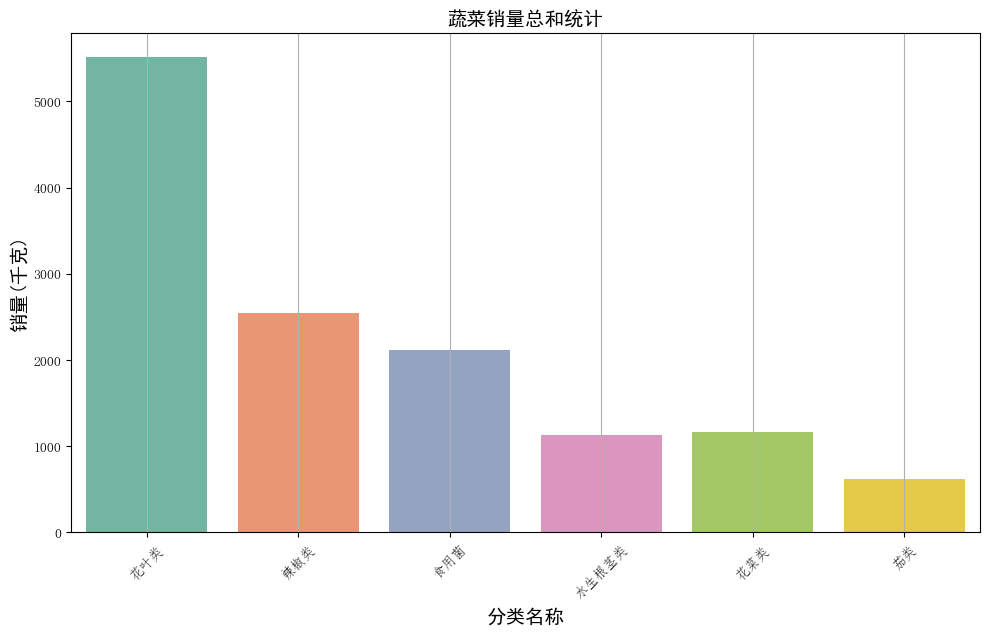
\includegraphics[width=1\textwidth]{1.png}
		\end{figure}
			\subsection{模型的建立}
		针对第一个问题,我们先对数据进行预处理,首先,我们将各个附件按照“单品编码”或“单品名称”组合成一张新的表格,其中包括了每种蔬菜销售信息,损耗率,批发价格等全部信息,这样有助于后期进一步对数据进行解读。
		
		首先我们以品类为单位,将五个品类蔬菜的销量在3年内的销量进行加总,分别得出五类蔬菜3年内的总销量,并画成了条形统计图。经过计算,花叶类蔬菜在销售中表现最出色,总销售量达到198,520.978千克。这类蔬菜可能包括各种绿叶蔬菜,如菠菜、生菜、菜心等。它们在市场中非常受欢迎,销售量较高。辣椒类蔬菜的销售量为91,588.629千克。这表明辣椒类蔬菜在市场上也有相当的销售份额,消费者可能对辛辣食物有较高的需求。食用菌类蔬菜的销售量为76,086.725千克。食用菌可能包括蘑菇、香菇等。尽管销售量低于花叶类和辣椒类,但它们仍然有一定的市场份额。水生根茎类蔬菜销售量为40,581.353千克。这类蔬菜包括像莲藕、芋头等水生植物的根茎部分。虽然销售量相对较低,但它们在市场上仍然有一定的存在。
		
		花菜类:花菜类蔬菜的销售量为41,766.451千克。这可能包括像西兰花、菜花等花头部分的蔬菜。尽管销售量较低,但它们仍然在市场上有市场份额。
		
		茄类:茄类蔬菜的销售量为22,431.782千克。这类蔬菜包括番茄、茄子等。销售量相对较低,但在某些时候可能会有季节性需求。
		
		这些数据描述了不同蔬菜分类的销售情况,显示出花叶类蔬菜在销售中表现最佳,而茄类蔬菜的销售量较低。这些信息有助于了解市场需求和销售趋势,为库存管理和定价策略提供了有价值的见解。
			\begin{figure}[H]
			\centering
			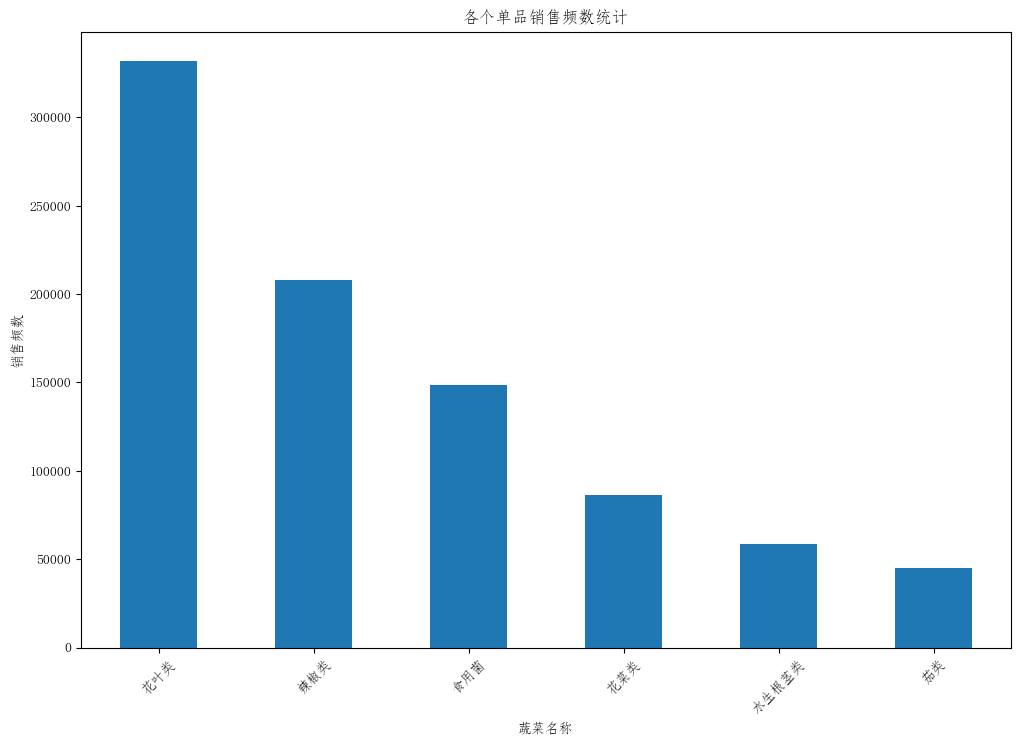
\includegraphics[width=1\textwidth]{2.png}
		\end{figure}
		由图可知,花叶类销售频数达到了331,968,是五种蔬菜中销售量最高的分类。这表明花叶类蔬菜在市场中非常受欢迎,可能是消费者日常膳食的重要组成部分。
		
		辣椒类蔬菜的销售频数为207,996,居于第二位。辣椒类蔬菜通常因其独特的风味和多用途性而备受欢迎,常用于各种烹饪中。
		
		食用菌的销售频数为148,424。这表明食用菌类蔬菜在市场中有一定的市场份额,可能被用于各种菜肴和料理。
		
		花菜类(Cauliflower):花菜类蔬菜的销售频数为86,570。虽然销售量较低,但仍然有一定市场存在,可能在特定菜肴或时段中更受欢迎。
		
		水生根茎类(Aquatic Roots and Tubers):水生根茎类蔬菜的销售频数为58,647,是五种蔬菜中销售量最低的分类。这类蔬菜可能在一些特定菜肴或地区中有市场需求。
		
		总的来说,销售频数数据反映了不同蔬菜分类的市场表现,有助于了解消费者的偏好和市场趋势。花叶类和辣椒类蔬菜在销售中表现出色,而其他分类虽然销售量较低,但仍然具有一定市场份额。这些信息对农产品供应链和市场营销策略的制定都具有重要的参考价值。
			\begin{figure}[H]
			\centering
			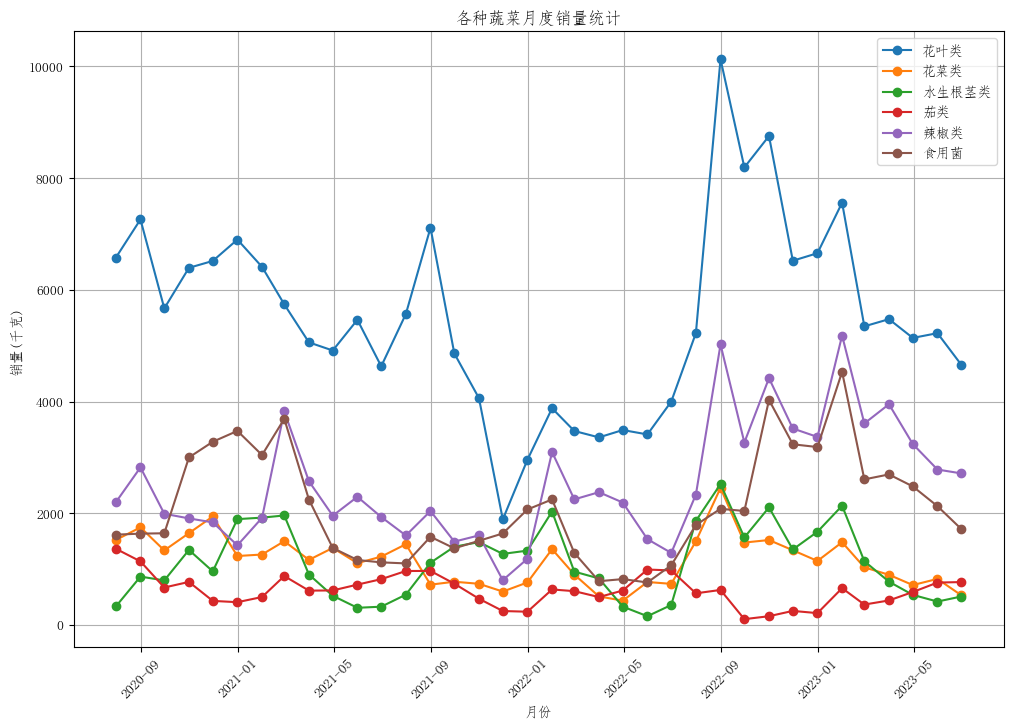
\includegraphics[width=1\textwidth]{3.jpg}
		\end{figure}
		
		此外,我们还在研究中发现数据存在相对时间周期性,本文选取小波分析算法,对数据进行处理
			\begin{figure}[H]
			\centering
			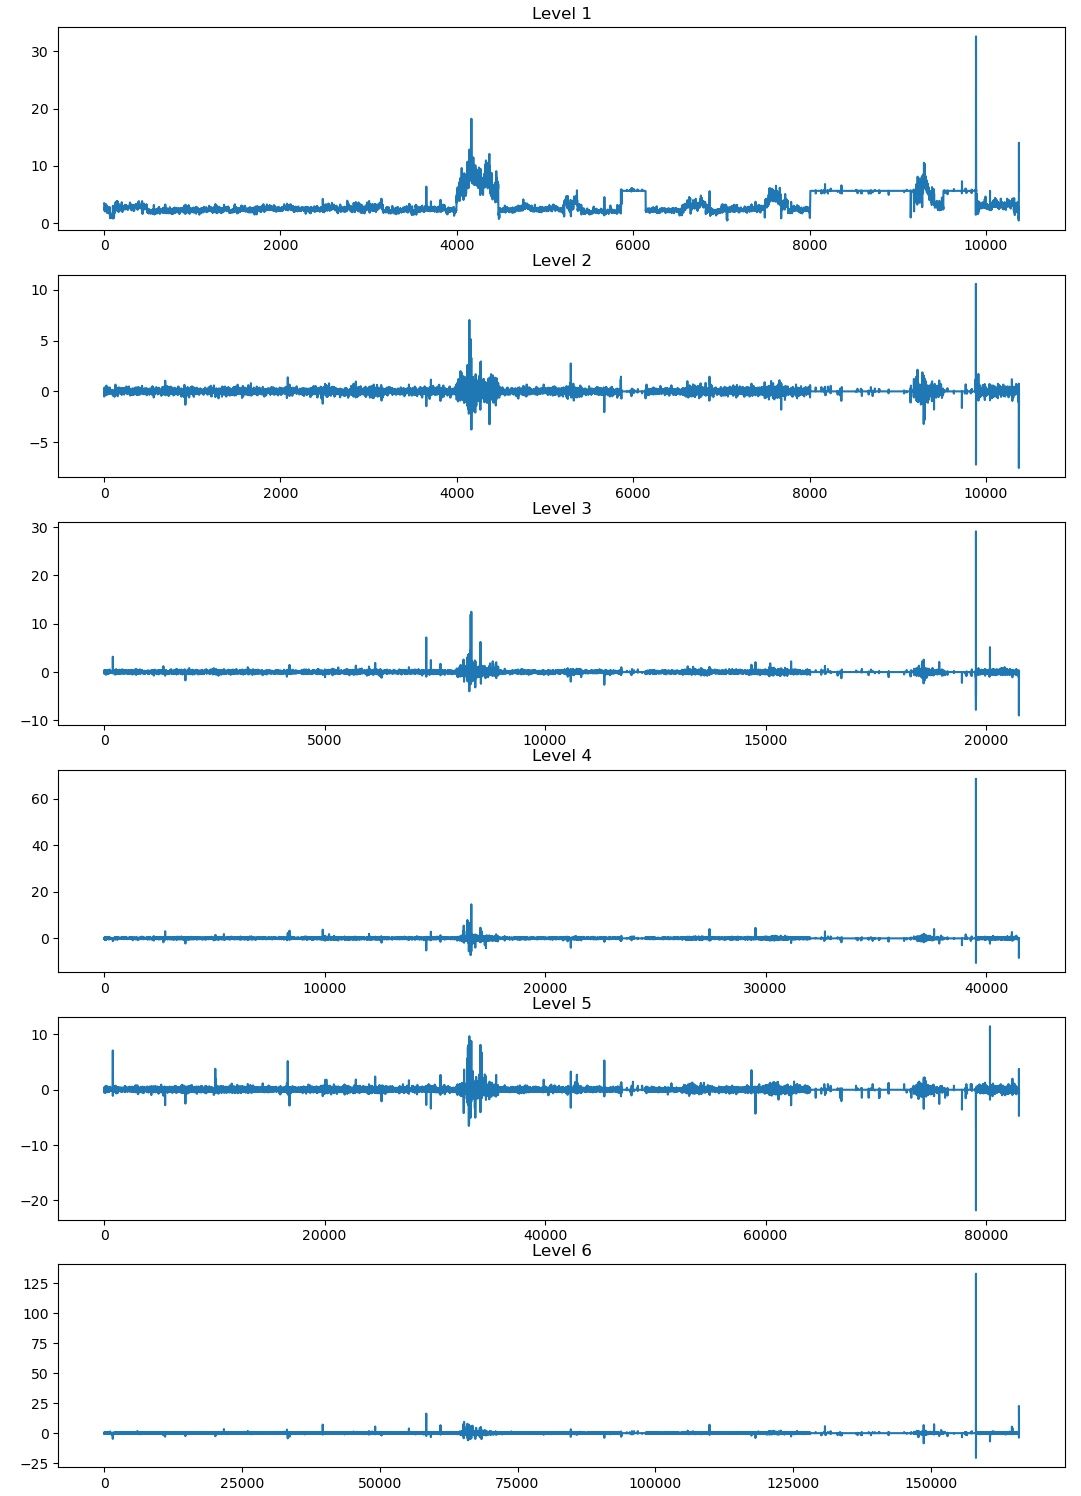
\includegraphics[width=1\textwidth]{小波.jpg}
		\end{figure}
		根据计算结果,我们可以看出,在Level2至Level5,分别代表年度到月度的波动情况,数据均存在周期性,而当数据在Level6,即当时间频率缩短到周,周期性消失。这证明了数据在月度层次即以上的周期性。
		
	根据提供的数据,我将进行对五种蔬菜类别:水生根茎类、花叶类、花菜类、茄类和辣椒类
	 在2020年7月1日至2023年6月30日三年时间内的月度销量的描述性统计分析。
	 
	首先,观察各个类别的销量变化趋势,水生根茎类的销量整体呈现稳定的趋势,但有轻微的波动,可能和季节性需求有关。花叶类的销量相较于其他类别较高,整体趋势稳定,有些许的上升趋势。花菜类的销量略低,但稳定,没有明显的上涨或下跌趋势。茄类的销量比较稳定,有轻微的上升趋势。辣椒类的销量有较大的波动性,可能与市场需求或季节性因素有关。
	
	在横向趋势比较中,花叶类的销量明显高于其他蔬菜类别,可能与其在各种菜肴中的普遍应用有关。辣椒类和水生根茎类的销量也较高,但略低于花叶类。花菜类和茄类的销量相对较低。
	
	对于提供的五类蔬菜三年内的月度销量数据(2020年7月1日至2023年6月30日),进行描述性统计分析如下:
	
	首先,让我们关注每种蔬菜分类的销量变化趋势:
	
	水生根茎类蔬菜的销量在三年内呈现了一定的波动,但总体上表现出稳步上升的趋势。销量的最高峰出现在2022年初,达到了约2,524.01千克,而最低点在2020年年末。这一分类的销量波动较小,总体来说,销量逐渐增加。花叶类蔬菜的销量在三年内经历了较大的波动。然而,总体趋势是逐渐上升的,尤其在最后一年有了显著的增长。销量的最高峰出现在2023年初,达到了约10,131.39千克。花菜类蔬菜的销量相对稳定,波动幅度较小。在三年内,销量总体上有所增长,但增长率较为缓慢。最高销量出现在2022年底,约为2,454.97千克。茄类蔬菜的销量在三年内有所波动,且总体销量较低。销量的峰值出现在2021年初,但在接下来的时间里波动较大。辣椒类蔬菜的销量在三年内经历了较大的波动,但总体呈上升趋势。最高销量出现在2023年初,约为5,182.98千克,而在早期的销量较低。食用菌类蔬菜的销量在三年内也有着显著的波动,但总体上呈增长趋势,特别是在最后一年增长明显。最高销量出现在2023年初,达到了约4,532.33千克。
	
	接下来,我们将进行各类蔬菜的横向趋势和相关度的比较:
	
	从销量趋势来看,花叶类、辣椒类和食用菌在三年内呈现出相对明显的增长趋势,而水生根茎类和花菜类的增长相对较为缓慢,茄类则波动幅度较大但总体趋势较为平稳。
	
	相关度比较:蔬菜分类之间的相关度可以通过相关系数来衡量。通过计算相关系数,我们可以发现哪些蔬菜分类之间存在正相关或负相关关系。例如,辣椒类和食用菌可能在某些时段表现出正相关关系,因为它们都在最后一年销量明显增加。另外,花叶类和花菜类的销量波动可能会受到相似的季节性影响,因此它们之间也可能存在一定的正相关关系。
	
	综合来看,这些蔬菜分类的销量表现各异,但总体趋势呈上升趋势,尤其是在最后一年。不同分类之间的相关性可能受到季节性、市场需求等因素的影响。这些分析结果对于决策制定、库存管理和市场预测都具有重要意义,有助于商家更好地了解市场动态并制定相应策略。
	
	花叶类、辣椒类和水生根茎类蔬菜在三年内的销量普遍较高,且销量变化趋势较稳定。花菜类和茄类的销量相对较低,且销量变化趋势与其他蔬菜类别相比较独立。以上分析可能与各类蔬菜的应用频率、消费者偏好及季节性因素有关,具体原因还需进一步深入研究。
		\begin{figure}[H]
		\centering
		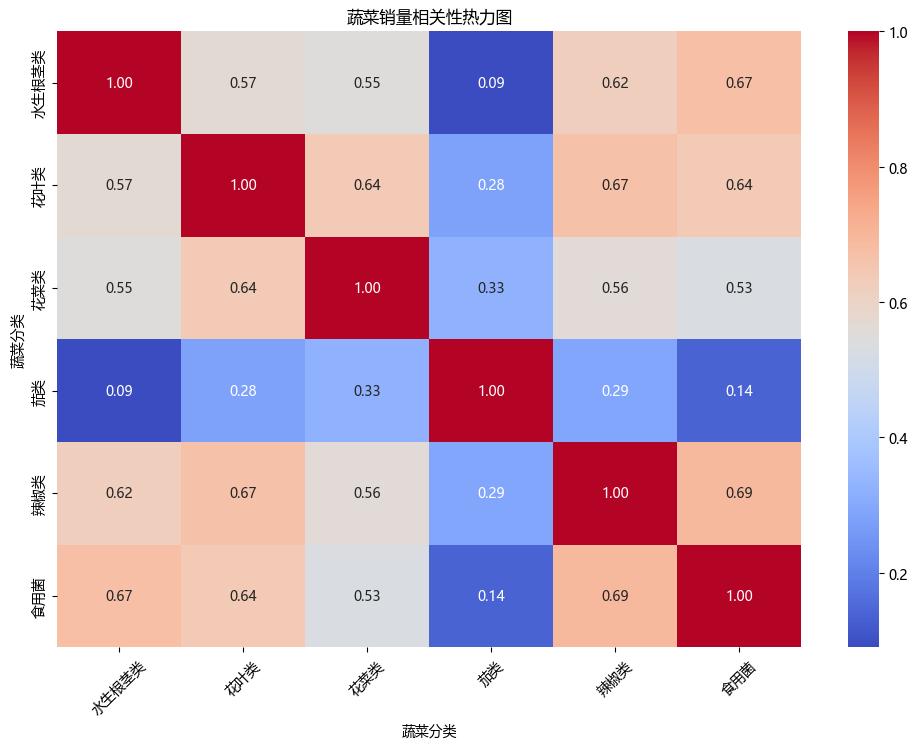
\includegraphics[width=1\textwidth]{4.png}
	\end{figure}
	根据相似性矩阵的分析,我们可以进一步深入了解不同蔬菜分类之间的关系和相似性,结合前面的销量和销售频数等数据,得出以下综合性分析:
	
	水生根茎类与花叶类之间存在较高的相关性,相关系数为0.57。这表示水生根茎类和花叶类的销售趋势在某种程度上相似,可能在某些市场条件下竞争或合作。水生根茎类与辣椒类和食用菌之间也存在较高的相关性,分别为0.62和0.67。这可能意味着在一些市场环境下,这些蔬菜分类之间存在潜在的销售关联。
	
	花叶类与辣椒类之间存在较高的相关性,相关系数为0.67。这表明花叶类和辣椒类的销售趋势可能受到相似的因素影响,可能具有一定的市场关联性。花叶类与食用菌之间也存在较高的相关性,相关系数为0.64。这可能意味着在某些市场中,花叶类和食用菌之间可能有一定的销售关联。
	
	花菜类与水生根茎类、花叶类和辣椒类之间存在一定的相关性,分别为0.55、0.64和0.56。这可能意味着花菜类与这些蔬菜分类之间在一些市场条件下可能存在一定的竞争或协作关系。
	
	茄类与其他蔬菜分类之间的相关性较低,相关系数都在0.29以下。这表示茄类与其他蔬菜分类之间的销售趋势不太相关,可能在市场上具有相对独立的地位。
	
	辣椒类与水生根茎类、花叶类和食用菌之间存在较高的相关性,分别为0.62、0.67和0.69。这表明辣椒类与这些蔬菜分类之间在某些市场环境下可能存在潜在的销售关联。
	
	食用菌与水生根茎类、花叶类和辣椒类之间存在较高的相关性,分别为0.67、0.64和0.69。这意味着食用菌与这些蔬菜分类之间在某些市场条件下可能有一定的销售关联性。
	
	通过这些相关性分析,我们可以更好地理解不同蔬菜分类之间的市场关系,有助于制定市场策略、供应链管理和产品推广等决策。不同分类之间的相似性和差异性也为进一步研究提供了有趣的线索。
		\begin{figure}[H]
		\centering
		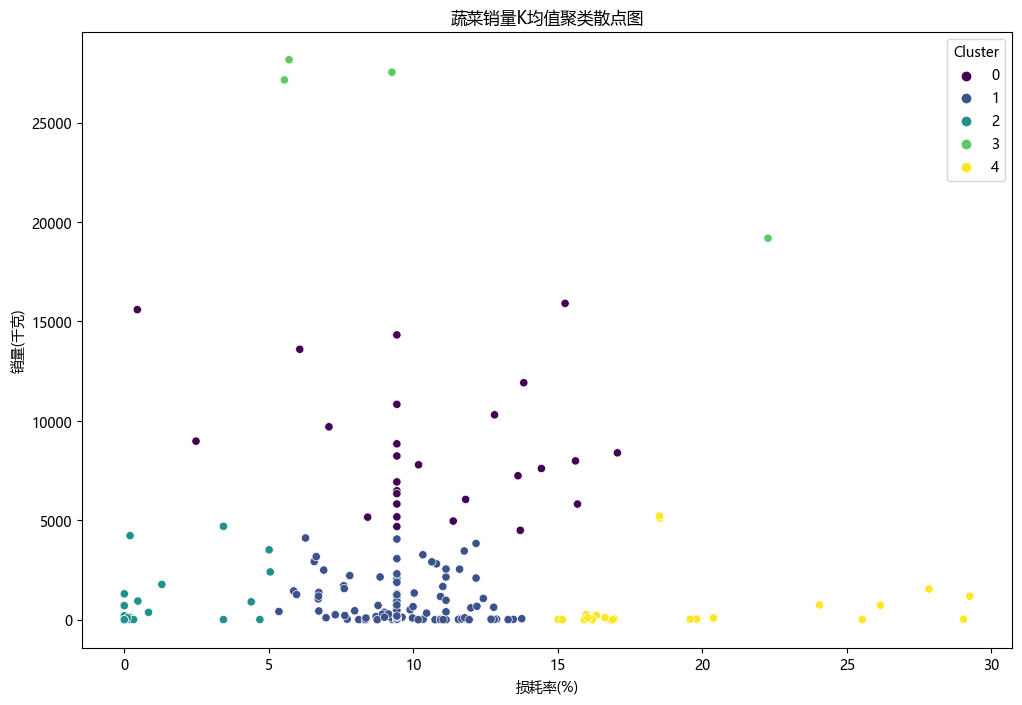
\includegraphics[width=1\textwidth]{5.png}
	\end{figure}
	以七彩椒(2)、云南油麦菜、大白菜为高销量低损耗群体,这一类单品在销量和损耗率方面表现出色,它们在市场上有很高的需求,并且能够有效地管理库存以减少损耗。这可能表明它们是热门单品,受欢迎程度高。这一类别的产品具有高销量和低损耗率,表明市场对其有强烈需求,并且库存管理良好。建议维持市场份额,甚至可以考虑适度提高价格,以提高利润率。由于销量较高,应定期监测库存水平,确保随时有足够的货物供应。根据销售趋势和季节性需求进行补货,以避免库存积压和供应不足。
	
	以姬菇(2)、黄白菜(2)、莲蓬(个)为代表低销量低损耗群体,这一类单品具有较低的销量和损耗率,它们可能在市场上不太受欢迎,或者需要更多的市场推广和管理努力来提高销售。根据市场反馈和需求,采取慎重的补货策略,避免库存积压。重点是了解潜在消费者需求并满足他们的期望。
	
	以青杭椒(1)、鲜藕带(袋)、黑油菜为代表的低销量高损耗群体:这一类单品虽然销量不高,但损耗率较高,这可能表明它们在市场上存在一定的需求,但需要改进库存管理和销售策略来减少损耗。根据市场需求和销售数据,采取小批量、定期的补货策略,以减少库存压力。
	
	以本地小毛白菜、枝江红菜苔、茼蒿(份)为代表的高销量高损耗群体销量高,但损耗率也相对较高。这可能是因为它们受欢迎,但需要更有效的库存管理,以减少浪费并提高利润。根据销售趋势定期补货,但重点是减少损耗,以提高盈利能力。
	
	云南生菜、小白菜、竹叶菜(份)等单品销量稳定,损耗率相对较低,它们在市场上具有一定的需求,并且有效地管理库存以减少损耗。根据销售情况和需求,采取合理的补货策略,避免库存积压或供应不足。
	需要注意的是,销售和补货策略不是一成不变的,应该根据市场变化、客户反馈和产品生命周期不断调整和优化。销售成功需要持续监测销售数据、库存水平以及竞争对手的动态,并与供应链伙伴和客户建立紧密的合作关系,以确保策略的有效实施。
	
	\section{问题二模型}
	\subsection{第一问}
	\subsubsection{数据准备}
	首先,我们需要收集关于问题的数据。在这个示例中,我们假设你有一个销售数据集,其中包括蔬菜品类、销售日期、销售量(总销量)和销售平均单价等信息。我们的目标是建立一个模型,根据销售日期和销售平均单价来预测销售量。在建立模型之前,我们需要对数据进行清洗和探索。这包括处理缺失值、异常值和重复数据,以确保数据的质量。我们还可以通过可视化和统计方法来探索数据的特征和分布,以更好地了解数据。
	
	在建立模型之前,我们对数据进行清洗和探索。这包括处理缺失值、异常值和重复数据,以确保数据的质量。我们还可以通过可视化和统计方法来探索数据的特征和分布,以更好地了解数据。
	
	在特征工程阶段,我们根据领域知识和数据分析的结果选择合适的特征。在这个问题中,我们选择了销售日期和销售平均单价作为特征。我们还可以考虑创建新的特征,如日期的季节性、假期等。
		\subsubsection{模型训练}
		在模型训练之前,我们将数据分为训练集和测试集。训练集用于训练模型,测试集用于评估模型的性能。通常,我们将大部分数据分配给训练集,而保留一小部分数据用于测试。在这个模型中,我们选择了随机森林回归模型。随机森林由多个决策树组成,每个决策树都对数据的一个子集进行训练。模型通过对多个决策树的预测结果进行平均或投票来提高预测的准确性。
		
		模型的训练过程包括以下步骤:
		
		- 从训练集中随机选择一个子集(有放回抽样)。
		
		- 构建一个决策树,通常在每个节点选择最佳特征来拆分数据。
		
		- 重复以上两个步骤多次,构建多个决策树。
		
		- 针对每个决策树的预测结果,进行平均或投票来获得最终的预测结果。
		
		模型的性能可以通过一些指标(如均方误差、R方值等)来评估。根据评估结果,我们调整了模型的超参数(如决策树数量、最大深度等)来提高模型的性能。
		
		运用模型我们最终得出一下回归结果:
				\begin{figure}[H]
			\centering
			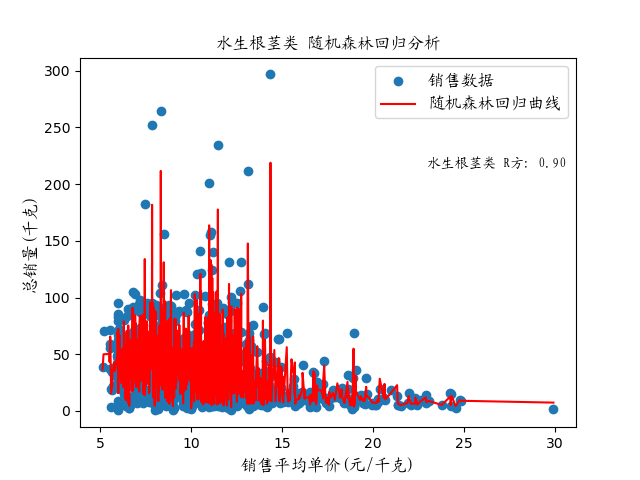
\includegraphics[width=1\textwidth]{p3.jpg}
		\end{figure}
		\subsection{问题二}
		\subsubsection{模型选择}
建立ARIMA(自回归滞后移动平均)模型是一种用于时间序列分析和预测的强大工具,通常用于预测未来的趋势和模式。在下面的文本中,我将详细解释如何建立ARIMA模型,包括数据准备、模型识别、参数估计和模型评估等步骤,以及其在现实中的应用和重要性。

ARIMA模型要求时间序列数据是平稳的。我们可以通过观察时间序列的图表和进行统计检验(如单位根检验)来确定是否需要进行差分操作以获得平稳性。

\subsubsection{自相关和偏自相关分析}

自相关和偏自相关函数图可以帮助我们确定ARIMA模型的阶数。自相关函数(ACF)和偏自相关函数(PACF)是时间序列的重要工具,用于识别自回归(AR)和移动平均(MA)的阶数。

确定了ARIMA模型的阶数,我们使用了最大似然估计或其他方法来估计模型的参数。这涉及到拟合ARIMA模型到训练数据,并确定模型的系数。
\subsubsection{模型检验}
建立ARIMA模型后,我们需要进行模型诊断来验证模型的质量。这包括检查模型的残差序列是否平稳和是否满足白噪声假设。我们可以使用Q-Q图和残差自相关函数图来检查这些假设。

模型性能可以通过一些指标来评估,包括均方根误差(RMSE)、平均绝对误差(MAE)和平均绝对百分比误差(MAPE)。我们运用这些指标了解模型的准确性和预测能力。
\subsubsection{数据结论}
根据模型我们得出如下规划
				\begin{figure}[H]
	\centering
	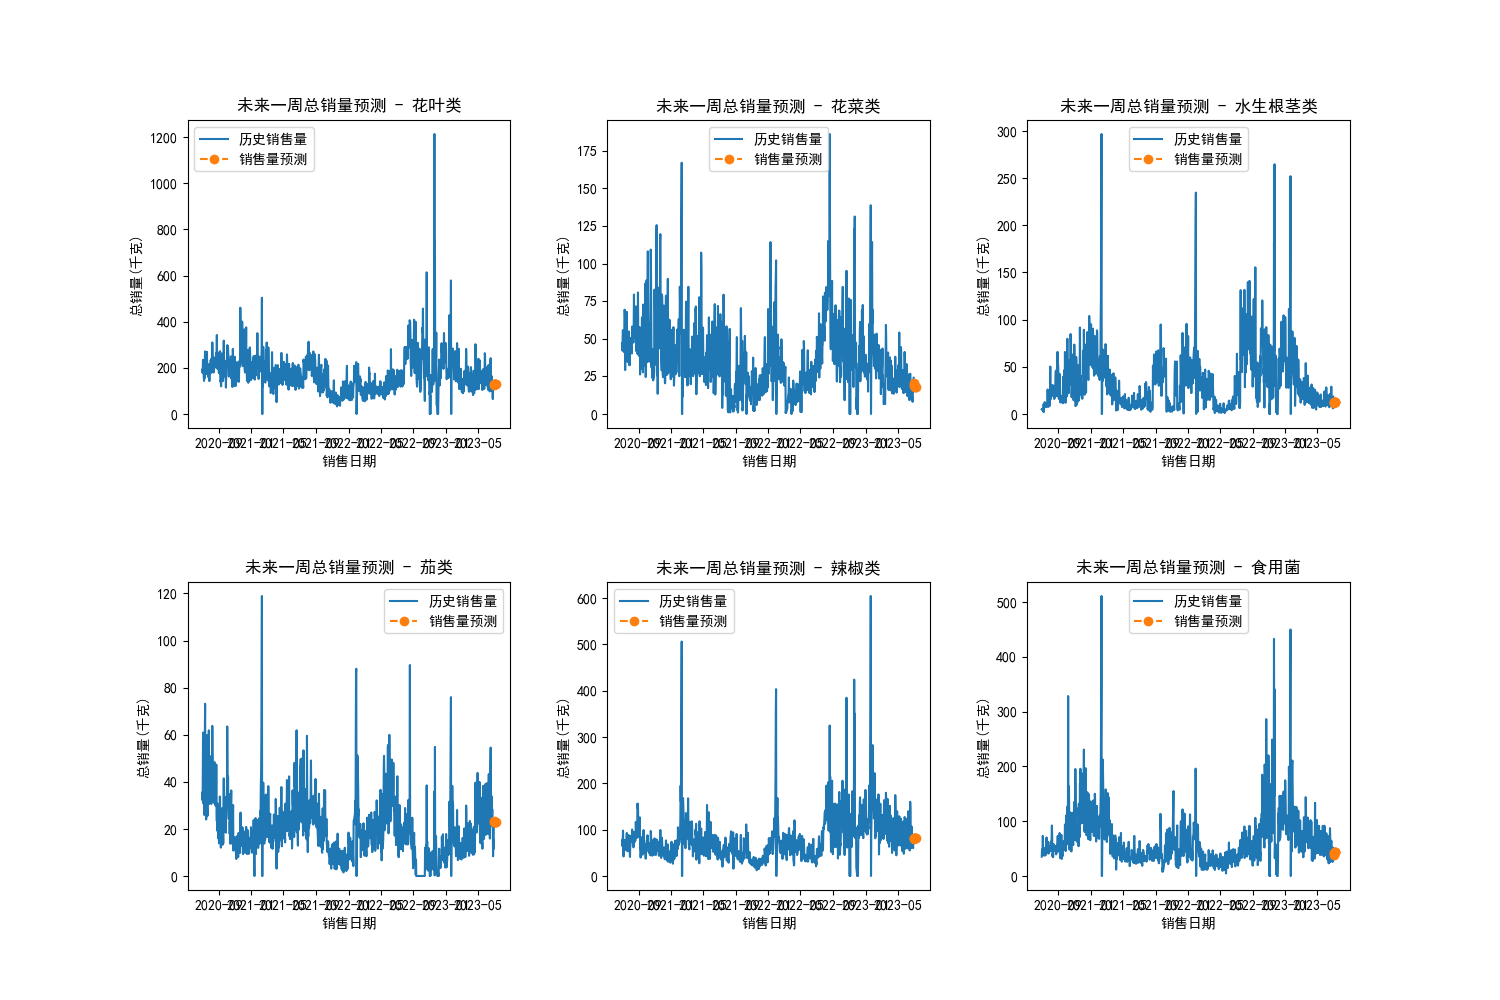
\includegraphics[width=1.1\textwidth]{q1.jpg}
\end{figure}

	\section{问题三模型}
		\subsection{数据准备}
		我们准备了以下数据:
		\begin{enumerate}
			\item 各个蔬菜品类的销售历史数据,包括销售量、销售价格等。
			\item 可售品种的信息,包括品类、历史销售情况、最小陈列量等。
			\item 定价策略相关的数据,如成本、利润率等。
			\item 商超的销售预测数据,以便预测未来一周的市场需求。
		\end{enumerate}
		
		\subsection{建立目标函数}
		我们的目标是最大化商超的收益,可以通过以下目标函数来表示:
		\begin{equation}
			Maximize Z = \sum_{i} (P_i \cdot Q_i - C_i \cdot Q_i)
		\end{equation}
		其中,$P_i$ 是商品 $i$ 的销售价格,$Q_i$ 是商品 $i$ 的补货量,$C_i$ 是商品 $i$ 的成本。
		
		\subsubsection{约束条件}
		\begin{enumerate}
			\item 总售卖单品数量限制在 27-33 个之间:这可以表示为
			\begin{equation}
				27 \leq \sum_{i} Y_i \leq 33
			\end{equation}
			其中,$Y_i$ 是商品 $i$ 是否被补货,取值为0或1。
			
			\item 单品补货量满足最小陈列量 2.5 千克的要求:这可以表示为
			\begin{equation}
				Q_i \geq 2.5 \cdot Y_i,      for all  i
			\end{equation}
			
			\item 商超销售预测需求:商超需要根据销售预测数据来满足市场需求,可以表示为
			\begin{equation}
				Q_i \leq     sales_i,     for all  i
			\end{equation}
			
			\item 非负性约束:补货量和价格都必须是非负的,可以表示为
			\begin{equation}
				Q_i \geq 0,      for all  i
			\end{equation}
			\begin{equation}
				P_i \geq 0,     for all  i
			\end{equation}
		\end{enumerate}
		
		\subsection{求解}
		将目标函数和约束条件组合成线性规划问题,并使用线性规划求解器(如PuLP、Gurobi等)来求解最优解。最优解将给出每个单品的补货量和定价策略,以最大化商超的收益。
		
		这个线性规划模型可以根据实际数据和需求进行调整和扩展,以更好地满足商超的具体情况。通过合理的数据准备和模型建立,商超可以制定出最优的单品补货计划和定价策略,以提高销售效益和最大化收益。
		
	
	\section{问题四模型}
\subsection{基于历史销售趋势的补货}
	销售趋势分析:首先,对历史销售数据进行深入分析,包括每周每天的销售量。根据这些数据,识别出销售高峰和低谷,特别是周末和周一的销售高峰。这有助于确定哪些蔬菜品类在不同时间段需求较高。
	库存警报系统:建立库存水平的警报系统,以确保库存不低于安全水平。当某一蔬菜品类的库存低于设定的警戒线时,系统应该自动触发补货流程。
	自动化补货流程:与供应商建立合作关系,使其能够在每天凌晨 3:00-4:00 之间供应所需数量的蔬菜。利用自动化订单系统,根据库存和销售数据生成订单,以减少人工干预。
\subsection{周一高销售需求的应对策略}
	周末前备货:考虑到周一通常有较高的销售需求,可在周末前增加库存。这可以通过在周五或周六的早晨进行额外的补货来实现。
	降低库存:在周二和周三逐渐降低库存水平,以避免过多的滞销库存。这可以通过减少进货数量来实现。
\subsection{库存管理和损失控制}	
	首进先出 (FIFO) 管理:确保库存中的商品按照先进先出原则管理,以降低产品损失。这对于保持蔬菜的新鲜度至关重要。
	库存定期检查:定期检查库存,及时识别品相变差或快过期的商品,并采取措施,如打折销售,以减少损失。
\subsection{数据分析和优化}
	实时销售监控:建立实时销售监控系统,以跟踪每日销售趋势。如果发现某一蔬菜品类的销售远超出预期,可以立即采取行动,增加补货数量。
	定期回顾:每周或每月回顾销售数据和库存情况,与供应商进行反馈,根据反馈不断优化补货策略。
\subsection{供应链优化}	
	供应商合作:建立稳定的供应链合作关系,确保供应商能够按时供货,并根据需求做出灵活调整。
	多源供应:考虑与多个供应商合作,以降低供应中断的风险,特别是针对季节性蔬菜。
	综合来看,这个详细的超市蔬菜补货策略包括了基于销售趋势的补货、库存管理、周一高销售需求的应对策略、数据分析和供应链优化。通过这些措施,超市可以更好地满足市场需求,减少库存损失,提高效益。然而,策略的成功也需要不断监控和反馈,以根据实际情况进行调整和优化。
	
	\section{模型的评价}
		\subsection{小波算法}
		
\subsubsection{模型的优点}
\begin{itemize}
	\item 多尺度分析: 分析通过不同尺度的小波基函数,可以同时捕捉信号或数据中的细节和整体特征。这使得它在分析具有多尺度特征的信号或数据时非常有用,如地震信号、生物医学图像等。
	\item 局部性质: 小波变换具有局部性质,每个小波基函数仅影响数据的局部区域,而不像傅立叶变换那样影响整个数据。这有助于更准确地定位信号中的特定特征,如信号中的突变点或频率成分。
	\item 分析与合成的平衡: 小波分析具有分析和合成的平衡性,允许从小波系数重构原始信号或数据。这种平衡性有助于信号去噪、图像恢复和数据恢复等应用。
	\item 分析与合成的平衡: 小波分析具有分析和合成的平衡性,允许从小波系数重构原始信号或数据。这种平衡性有助于信号去噪、图像恢复和数据恢复等应用。
\end{itemize}
\subsubsection{模型的缺点}
\begin{itemize}
	\item 复杂性: 小波分析的数学理论和算法相对较复杂,需要一定的数学背景和技能才能正确应用。这可能使得对小波分析的学习和应用具有一定的门槛。
	\item 选择小波基函数: 选择合适的小波基函数对于小波分析至关重要。不同的基函数适用于不同类型的数据,因此需要对数据特性有一定的先验知识或尝试多种基函数。
	\item 丧失全局信息: 小波分析的局部性质也是其缺点之一,它可能导致在一些情况下丧失全局信息。例如,在一些信号中,小波分析可能无法准确捕捉整体趋势。
\end{itemize}

		\subsection{聚类分析}
\subsubsection{模型的优点}
\begin{itemize}
	\item 模式发现: 聚类分析可以帮助识别数据集中的隐藏模式和结构。通过将相似的数据点分组到同一个簇中,可以更好地理解数据的内在关系和组织。
	\item 无监督学习: 聚类是一种无监督学习方法,不需要预先标记的训练数据。这意味着它可以应用于各种数据类型,包括那些没有先验信息的数据集。
	\item 数据降维: 聚类分析有助于减少数据集的维度,将复杂的数据集简化为更容易理解和处理的形式。这对于可视化和进一步分析非常有用。
	\item 异常检测: 聚类可以用于检测异常值,因为异常数据点通常与其他数据点有明显的差异,可能被分配到单独的簇中。
\end{itemize}
\subsubsection{模型的缺点}
\begin{itemize}
	\item 初始条件敏感: 聚类算法的结果可能高度依赖于初始条件和随机初始化。不同的初始值可能导致不同的聚类结果,需要多次运行算法来获取稳定的结果。
	\item 簇的数量选择: 通常需要预先指定要分为多少个簇,但在实际应用中,簇的数量可能不容易确定,选择不当可能导致不准确的聚类。
	\item 对异常值敏感: 聚类算法对异常值敏感,异常值可能会影响簇的形成和结果的准确性。
\end{itemize}
	
		\subsection{ARIMA}
\subsubsection{模型的优点}
\begin{itemize}
	\item 简单性: ARIMA模型是一种相对简单的时间序列模型。它基于几个基本概念,包括自回归(AR)、差分(I)和移动平均(MA),这些概念相对容易理解。
	\item 良好的预测性能: 当时间序列数据满足一定的条件时,ARIMA模型可以提供相当准确的预测结果。这对于制定业务决策和计划非常有用。
	\item 可解释性: ARIMA模型生成的预测结果可以被解释和理解。它们通常基于过去的观察结果和趋势,因此能够为未来的趋势提供合理的解释。
	\item 稳定性: ARIMA模型对于时间序列数据中的季节性和趋势性具有较好的稳定性,能够有效地捕捉这些特征。
	\item 自动建模: ARIMA模型中的参数估计和模型选择通常是自动完成的,无需用户干预。这使得ARIMA模型对于不具备专业时间序列分析知识的人来说也可以使用。
\end{itemize}
\subsubsection{模型的缺点}
\begin{itemize}
	\item 对数据要求高: ARIMA模型要求输入的时间序列数据是平稳的,即均值和方差保持恒定。如果数据不满足这一条件,就需要进行差分操作,这可能导致数据信息的丢失。
	\item 不适用于非线性数据: ARIMA模型假设时间序列数据是线性的,因此对于非线性的数据,它的预测能力会受到限制。如果数据包含复杂的非线性关系,ARIMA模型可能无法捕捉到这些关系。
	\item 对异常值敏感: ARIMA模型对异常值(离群值)非常敏感,异常值可能对模型的拟合和预测产生不良影响。
\end{itemize}
	%参考文献
	%	\begin{thebibliography}{9}%宽度9
	%		\bibitem[1]{liuhaiyang2013latex}
	%		刘海洋.
	%		\newblock \LaTeX {}入门\allowbreak[J].
	%		\newblock 电子工业出版社, 北京, 2013.
	%		\bibitem[2]{mathematical-modeling}
	%		全国大学生数学建模竞赛论文格式规范 (2020 年 8 月 25 日修改).
	%		\bibitem{3} \url{https://www.latexstudio.net}
	%	\end{thebibliography}
	
	\section{参考文献}
[1]苏丰睿,穆伟伟,赵宣茗等.一种划分聚类k值与中心初始化改进方法[J/OL].计算机工程:1-11[2023-09-10].DOI:10.19678/j.issn.1000-3428.0065422.

[2]张黎,王振全.基于小波分析与支持向量机控制图混合模式识别[J].郑州航空工业管理学院学报,2023,41(04):64-72.DOI:10.19327/j.cnki.zuaxb.1007-9734.2023.04.008.

[3]谢杰成,张大力,徐文立.小波图象去噪综述[J].中国图象图形学报,2002(03):3-11.

[4]陈弘,周宗放,陈军.生鲜农产品生长增值期内库存补货策略[J].系统工程,2012,30(01):91-96.

[5]刘海滨. 连锁超市采购管理研究[D].天津大学,2004.

[6]李春涵,吴宝宏.连锁超市存货成本控制问题与建议探究[J].中国管理信息化,2019,22(20):14-15.

[7]王森,刘琛,邢帅杰.K-means聚类算法研究综述[J].华东交通大学学报,2022,39(05):119-126.DOI:10.16749/j.cnki.jecjtu.20220914.001.

[8]袁紫微,李洋.基于Flexsim的中小型超市补货优化研究[J].物流科技,2014,37(10):72-76.DOI:10.13714/j.cnki.1002-3100.2014.10.023.

[9]徐艺萌. L生鲜果蔬连锁超市库存管理研究[D].昆明理工大学,2019.DOI:10.27200/d.cnki.gkmlu.2019.000182.

[10]郭英,冯茗杨,孙玉曦等.聚类阈值结合动态K值的蓝牙室内定位算法[J].测绘科学,2019,44(11):184-188+194.DOI:10.16251/j.cnki.1009-2307.2019.11.027.

	
	\newpage
	%附录
	\begin{appendices}
		\section{文件列表}
		% Table generated by Excel2LaTeX from sheet 'Sheet1'
		\begin{table}[htbp]
			\centering
			\caption{Add caption}
			\begin{tabularx}{\textwidth}{@{}c *1{>{\centering\arraybackslash}X}@{}}
				\toprule[1.5pt]
				文件名   & 文件描述 \\
				\midrule
				数据\_处理后(剔除).xlsx & 附件数据处理 \\
				ARIMA.py & ARIMA算法 \\
				随机森林代码.py & 随机森林算法 \\
				回归.py & 回归求解 \\
				非线性.py & 非线性方程 \\
				小波分析.py & 小波分析算法 \\
				\bottomrule
			\end{tabularx}%
			\label{tab:addlabel}%
		\end{table}%
	\section{代码}
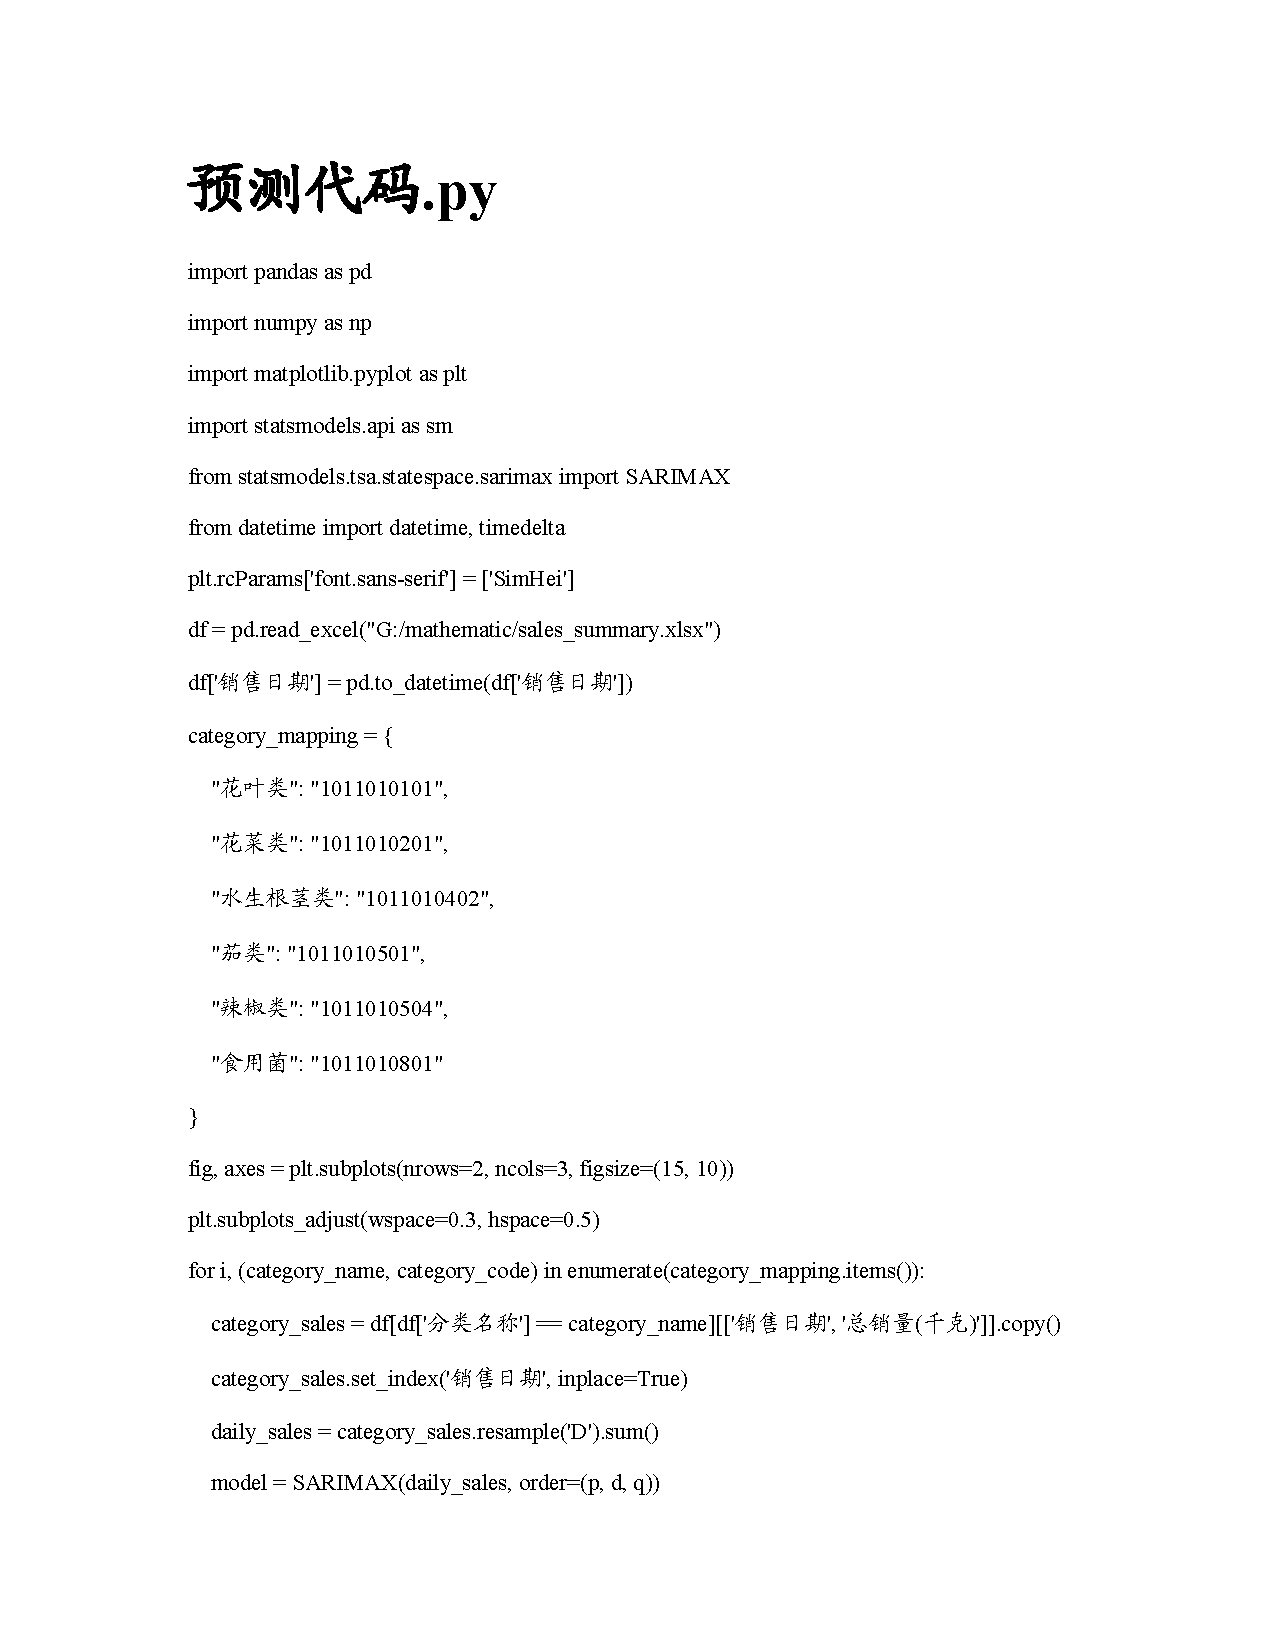
\includepdf[pages={1}]{code.pdf}           
\includepdf[pages={2}]{code.pdf}     
\includepdf[pages={3}]{code.pdf}     
\includepdf[pages={4}]{code.pdf}     
\includepdf[pages={5}]{code.pdf}     
\includepdf[pages={6}]{code.pdf}     
\includepdf[pages={7}]{code.pdf}     
\includepdf[pages={8}]{code.pdf}     
\includepdf[pages={9}]{code.pdf}     
\includepdf[pages={10}]{code.pdf}     
\includepdf[pages={11}]{code.pdf}     
\includepdf[pages={12}]{code.pdf}     
\includepdf[pages={13}]{code.pdf}     
\includepdf[pages={14}]{code.pdf}     
\includepdf[pages={15}]{code.pdf}     
\includepdf[pages={16}]{code.pdf}     
\includepdf[pages={17}]{code.pdf}     
\includepdf[pages={18}]{code.pdf}     
\includepdf[pages={19}]{code.pdf}     
\includepdf[pages={20}]{code.pdf}     
	\end{appendices}
	
\end{document} 